%!TEX root = modelguide.tex

\chapter{Mechanical Models II}
\label{MechModelsII:sec}

This section provides additional material on building basic
multibody-type mechanical models.

\section{Simulation control properties}

Both \javaclass[artisynth.core.workspace]{RootModel} and
\javaclass[artisynth.core.mechmodels]{MechModel} contain properties
that control the simulation behavior. One of the most important of
these is {\tt maxStepSize}. By default, simulation proceeds using the
{\tt maxStepSize} value defined for the root model. A {\tt MechModel}
(or any other type of {\tt Model}) contained in the root model's {\tt
models} list may also request a smaller step size by specifying a
smaller value for its own {\tt maxStepSize} property.  For all models,
the {\tt maxStepSize} may be set and queried using
%
\begin{lstlisting}[]
  void setMaxStepSize (double maxh);
  double getMaxStepSize();
\end{lstlisting}
%

Another important simulation property is {\tt integrator} in {\tt
MechModel}, which determines the type of integrator used for the
physics simulation. The value type of this property is the enumerated
type {\tt MechSystemSolver.Integrator}, for which the following values
are currently defined:

\begin{description}

\item[ForwardEuler]\mbox{}

First order forward Euler integrator. Unstable for stiff systems.

\item[SymplecticEuler]\mbox{}

First order symplectic Euler integrator, more energy conserving
that forward Euler. Unstable for stiff systems.

\item[RungeKutta4]\mbox{}

Fourth order Runge-Kutta integrator, quite accurate but also unstable
for stiff systems.

\item[ConstrainedBackwardEuler]\mbox{}

First order backward order integrator. Generally stable for stiff systems.

\item[Trapezoidal]\mbox{}

Second order trapezoidal integrator. Generally stable for stiff
systems, but slightly less so than {\tt ConstrainedBackwardEuler}.

\end{description}

The term ``Unstable for stiff systems'' means that the integrator is
likely to go unstable in the presence of ``stiff'' systems, which
typically include systems containing finite element models, unless the
simulation step size is set to an extremely small value.  The default
value for {\tt integrator} is {\tt ConstrainedBackwardEuler}.

\begin{sideblock}
Stiff systems tend to arise in models containing interconnected
deformable elements, for which the step size should not exceed the
propagation time across the smallest element, an effect known as the
Courant-Friedrichs-Lewy (CFL) condition. Larger stiffness and damping
values decrease the propagation time and hence the allowable step
size.
\end{sideblock}

Another {\tt MechModel} simulation property is {\tt stabilization},
which controls the stabilization method used to correct drift from
position constraints and correct interpenetrations due to collisions.
The value type of this property value is the enumerated type {\tt
MechSystemSolver.PosStabilization}, which presently has two values:

\begin{description}

\item[GlobalMass]\mbox{}

Uses only a diagonal mass matrix for the MLCP that is solved to
determine the position corrections. This is the default method.

\item[GlobalStiffness]\mbox{}

Uses a stiffness-corrected mass matrix for the MLCP that is solved to
determine the position corrections. Slower than {\tt GlobalMass}, but
more likely to produce stable results, particularly for
problems involving FEM collisions.

\end{description}

\section{Units}
\label{sec:mechii:units}

ArtiSynth is primarily ``unitless'', in the sense that it does not
define default units for the fundamental physical quantities of time,
length, and mass. Although time is
generally understood to be in seconds, and often declared as such in
method arguments and return values, there is no hard requirement that
it be interpreted as seconds. There are no assumptions at all
regarding length and mass. Some components may have default parameter
values that reflect a particular choice of units, such as {\tt
MechModel}'s default gravity value of $(0, 0, -9.8)^T$, which is
associated with the MKS system, but these values can always be
overridden by the application.

Nevertheless, it is important, and up to the application developer to
ensure, that units be {\it consistent}. For example, if one decides to
switch length units from meters to centimeters (a common choice),
then all units involving length will have to be scaled appropriately.
For example, density, whose fundamental units are $m/d^3$, where $m$ is mass and
$d$ is distance, needs to be scaled by $1/100^3$, or $0.000001$, when
converting from meters to centimeters.

Table \ref{Units:tab} lists a number of common physical quantities
used in ArtiSynth, along with their associated fundamental units.

\begin{table}
\begin{center}
\begin{tabular}{|lll|}
\hline
unit & fundamental units & \\
\hline
time                    & $t$ & \\
distance                & $d$ & \\
mass                    & $m$ & \\
velocity                & $d/t$ & \\
acceleration            & $d/t^2$ & \\
force                   & $m d/t^2$ & \\
work/energy             & $m d^2/t^2$& \\
torque                  & $m d^2/t^2$ & same as energy (somewhat counterintuitive)\\
angular velocity        & $1/t$ & \\
angular acceleration    & $1/t^2$ & \\
rotational inertia      & $m d^2$ & \\
pressure                & $m/(d t^2)$ & \\
Young's modulus         & $m/(d t^2)$ & \\
Poisson's ratio         & 1 & no units; it is a ratio \\
density                 & $m/d^3$ & \\
linear stiffness        & $m/t^2$ & \\
linear damping          & $m/t$ & \\
rotary stiffness        & $m d^2/t^2$ & same as torque \\
rotary damping          & $m d^2/t$ & \\
mass damping            & $1/t$ & used in FemModel \\
stiffness damping       & $t$ & used in FemModel \\
\hline
\end{tabular}
\end{center}
\caption{Physical quantities and their representation in terms of the
fundamental units of mass ($m$), distance ($d$), and time ($t$).}
\label{Units:tab}
\end{table}

\subsection{Scaling units}

For convenience, many ArtiSynth components, including {\tt MechModel},
implement the interface
\javaclass[artisynth.core.util]{ScalableUnits}, which
provides the following methods for scaling mass and distance units:
%
\begin{lstlisting}[]
  scaleDistance (s);    // scale distance units by s
  scaleMass (s);        // scale mass units by s
\end{lstlisting}
%
A call to one of these methods should cause all physical quantities
within the component (and its descendants) to be
scaled as required by the fundamental unit relationships
as shown in Table \ref{Units:tab}.

Converting a {\tt MechModel} from meters to centimeters can therefore be
easily done by calling 
%
\begin{lstlisting}[]
   mech.scaleDistance (100);
\end{lstlisting}
%
As an example, adding the following code to the end of the {\tt build()}
method in {\tt RigidBodySpring} (Section \ref{RigidBodySpringExample:sec})
%
\begin{lstlisting}[]
   System.out.println ("length=" + spring.getLength());
   System.out.println ("density=" + box.getDensity());
   System.out.println ("gravity=" + mech.getGravity());
   mech.scaleDistance (100);
   System.out.println ("");
   System.out.println ("scaled length=" + spring.getLength());
   System.out.println ("scaled density=" + box.getDensity());
   System.out.println ("scaled gravity=" + mech.getGravity());
\end{lstlisting}
%
will scale the distance units by 100 and print the values of various
quantities before and after scaling. The resulting output is:
%
\begin{lstlisting}[]
   length=0.5
   density=20.0
   gravity=0.0 0.0 -9.8

   scaled length=50.0
   scaled density=2.0E-5
   scaled gravity=0.0 0.0 -980.0
\end{lstlisting}
%

\begin{sideblock}
It is important not to confuse scaling units with scaling the actual
geometry or mass. Scaling units should change all physical
quantities so that the simulated behavior of the model remains
unchanged.  If the distance-scaled version of {\tt RigidBodySpring}
shown above is run, it should behave exactly the same as the
non-scaled version.
\end{sideblock}

%\section{Multi-point springs}
%OPTIONAL
%\subsection{Operation}
%\subsection{Example: A single multi-point spring}

%\begin{figure}[ht]
%\begin{center}
%\iflatexml
% 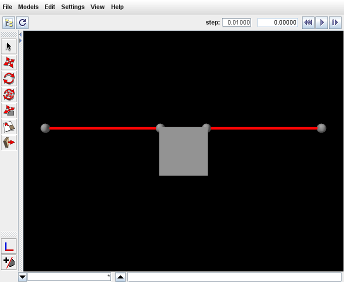
\includegraphics[]{images/MultiPointSpring}
%\else
% 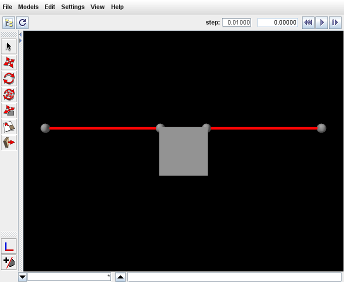
\includegraphics[width=3.75in]{images/MultiPointSpring}
%\fi
%\end{center}
%\caption{MultiPointSpring model loaded into ArtiSynth.}
%\label{MultiPointSpring:fig}
%\end{figure}
%
%A simple model showing a multi-point spring is defined in
%%
%\begin{verbatim}
%  artisynth.demos.tutorial.MultiPointSpring
%\end{verbatim}
%

% MultiPointSpring

\section{Render properties}
\label{RenderProperties:sec}

All ArtiSynth components that are renderable maintain a property {\tt
renderProps}, which stores a
\javaclass[maspack.render]{RenderProps} object that contains a number
of subproperties used to control an object's rendered appearance.

In code, the {\tt renderProps} property for an object can be set or
queried using the methods
%
\begin{lstlisting}[]
  setRenderProps (RenderProps props); // set render properties
  RenderProps getRenderProps();       // get render properties (read-only)
\end{lstlisting}
%
Render properties can also be set in the GUI by selecting one or more
components and the choosing {\sf Set render props ...}  in the
right-click context menu. More details on setting render properties
through the GUI can be found in the section ``Render properties'' in the
\href{\artisynthDocBase/html/uiguide/uiguide.html}{
ArtiSynth User Interface Guide}.

For many components, the default value of {\tt renderProps} is {\tt
null}; i.e., no {\tt RenderProps} object is assigned by default and
render properties are instead inherited from ancestor components
further up the hierarchy. The reason for this is because {\tt
RenderProps} objects are fairly large (many kilobytes), and so
assigning a unique one to every component could consume too much
memory. Even when a {\tt RenderProps} object is assigned, most of its
properties are inherited by default, and so only those properties
which are explicitly set will differ from those specified in ancestor
components.

\subsection{Render property taxonomy}

In general, the properties in {\tt RenderProps} are used to control
the color, size, and style of the three primary rendering
primitives: faces, lines, and points. Table \ref{RenderProps:tab}
contains a complete list. Values for the {\tt shading}, {\tt
faceStyle}, {\tt lineStyle} and {\tt pointStyle} properties are
defined using the following enumerated types:
\javaclass[maspack.render]{Renderer\$Shading}, 
\javaclass[maspack.render]{Renderer\$Faces}, 
\javaclass[maspack.render]{Renderer\$PointStyle}, 
and 
\javaclass[maspack.render]{Renderer\$LineStyle}.
Colors are specified using {\tt java.awt.Color}.

\begin{table}
\begin{center}
\begin{tabular}{|lll|}
\hline property & purpose & usual default value \\ \hline
%Generic properties:
visible & whether or not the component is visible & {\tt true} \\
alpha & transparency for diffuse colors (range 0 to 1) & 1 (opaque) \\
shading & shading style: 
({\tt FLAT}, {\tt SMOOTH}, {\tt METAL}, {\tt NONE}) & {\tt FLAT}\\
shininess & shininess parameter (range 0 to 128) & 32 \\
specular & specular color components & {\tt null} \\
%Face related properties &
\hline
faceStyle &
which polygonal faces are drawn ({\tt FRONT}, {\tt BACK},
{\tt FRONT\_AND\_BACK}, {\tt NONE}) & {\tt FRONT} \\
faceColor &
diffuse color for drawing faces & {\tt GRAY} \\
backColor &
diffuse color used for the backs of faces. 
If {\tt null}, {\tt faceColor} is used. & {\tt null} \\
drawEdges & hint that polygon edges should be drawn explicitly & {\tt false} \\
%Texture mapping properties &
\hline
colorMap & color mapping properties 
(see Section \ref{TextureMapping:sec}) & {\tt null} \\
normalMap & normal mapping properties 
(see Section \ref{TextureMapping:sec}) & {\tt null} \\
bumpMap & bump mapping properties 
(see Section \ref{TextureMapping:sec}) & {\tt null} \\
% Edge related properties &
\hline
edgeColor & diffuse color for edges & {\tt null} \\
edgeWidth & edge width in pixels & 1 \\
% Line related properties &
\hline
lineStyle: &
how lines are drawn ({\tt CYLINDER}, {\tt LINE}, or {\tt SPINDLE}) & 
{\tt LINE} \\
lineColor & diffuse color for lines & {\tt GRAY} \\
lineWidth & width in pixels when {\tt LINE} style is selected & 1 \\
lineRadius & radius when {\tt CYLINDER} or {\tt SPINDLE} style is selected &
1 \\
% Point related properties &
\hline
pointStyle & how points are drawn ({\tt SPHERE} or {\tt POINT}) & {\tt POINT} \\
pointColor & diffuse color for points & {\tt GRAY} \\
pointSize & point size in pixels when {\tt POINT} style is selected & 1 \\
pointRadius & sphere radius when {\tt SPHERE} style is selected & 1 \\
\hline
\end{tabular}
\end{center}
\caption{Render properties and their default values.}
\label{RenderProps:tab}
\end{table}

To increase and improve their visibility, both the line and point
primitives are associated with styles ({\tt CYLINDER}, {\tt
SPINDLE}, and {\tt SPHERE}) that allow them to be rendered using 3D
surface geometry.

Exactly how a component interprets its render properties is up to the
component (and more specifically, up to the rendering method for that
component).  Not all render properties are relevant to all components,
particularly if the rendering does not use all of the rendering
primitives. For example,
\javaclass[artisynth.core.mechmodels]{Particle} components use only
the point primitives and
\javaclass[artisynth.core.mechmodels]{AxialSpring} components use only
the line primitives. For this reason, some components use subclasses
of {\tt RenderProps}, such as
\javaclass[maspack.render]{PointRenderProps} and
\javaclass[maspack.render]{LineRenderProps}, that expose only a subset
of the available render properties. All renderable components provide
the method
\javamethod[maspack.render.HasRenderProps]{createRenderProps()} that
will create and return a {\tt RenderProps} object suitable for that
component.

\subsection{Setting render properties}
\label{SettingRenderProperties:sec}

When setting render properties, it is important to note that
the value returned by
\javamethod[maspack.render.HasRenderProps]{getRenderProps()} 
should be treated as {\it read-only} and should {\it not}
be used to set property values.
For example, applications should {\it not} do the
following:
\begin{lstlisting}[]
   particle.getRenderProps().setPointColor (Color.BLUE);
\end{lstlisting}
%
This can cause problems for two reasons. First, {\tt getRenderProps()}
will return {\tt null} if the object does not currently have a {\tt
RenderProps} object. Second, because {\tt RenderProps} objects are
large, ArtiSynth may try to share them between components, and so by
setting them for one component, the application my inadvertently set
them for other components as well.

Instead, {\tt RenderProps} provides a static method for each property
that can be used to set that property's value for a specific
component.  For example, the correct way to set {\tt pointColor} is
%
\begin{lstlisting}[]
   RenderProps.setPointColor (particle, Color.BLUE);
\end{lstlisting}
%

One can also set render properties by calling
\javamethod*[maspack.render.HasRenderProps]{setRenderProps()} with a
predefined {\tt RenderProps} object as an argument. This is useful for
setting a large number of properties at once:
%
\begin{lstlisting}[]
   RenderProps props = new RenderProps();
   props.setPointColor (Color.BLUE);
   props.setPointRadius (2);
   props.setPointStyle (RenderProps.PointStyle.SPHERE);

   ...

   particle.setRenderProps (props);
\end{lstlisting}

For setting each of the color properties within {\tt RenderProps},
one can use either {\tt Color} objects or {\tt float[]} arrays
of length 3 giving the RGB values. Specifically, there
are methods of the form
%
\begin{lstlisting}[]
   props.setXXXColor (Color color)
   props.setXXXColor (float[] rgb)
\end{lstlisting}
%
as well as the static methods
%
\begin{lstlisting}[]
   RenderProps.setXXXColor (Renderable r, Color color)
   RenderProps.setXXXColor (Renderable r, float[] rgb)
\end{lstlisting}
%
where {\tt XXX} corresponds to {\tt Point}, {\tt Line}, {\tt Face},
{\tt Edge}, and {\tt Back}. For {\tt Edge} and {\tt Back}, both {\tt
color} and {\tt rgb} can be given as {\tt null} to clear the indicated
color. For the specular color, the associated methods are
%
\begin{lstlisting}[]
   props.setSpecular (Color color)
   props.setSpecular (float[] rgb)
   RenderProps.setSpecular (Renderable r, Color color)
   RenderProps.setSpecular (Renderable r, float[] rgb)
\end{lstlisting}
%

\begin{sideblock}
Note that even though components may use a subclass of {\tt
RenderProps} internally, one can always use the base {\tt RenderProps}
class to set values; properties which are not relevant to the
component will simply be ignored.
\end{sideblock}

Finally, as mentioned above, render properties are inherited.  Values
set high in the component hierarchy will be inherited by descendant
components, unless those descendants (or intermediate components)
explicitly set overriding values.  For example, a {\tt MechModel}
maintains its own {\tt RenderProps} (and which is never null). Setting
its {\tt pointColor} property to {\tt RED} will cause {\it all}
point-related components within that {\tt MechModel} to be rendered as
red {\it except} for components that set their {\tt pointColor} to a
different property.

There are typically three levels in a {\tt MechModel} component
hierarchy at which render properties can be set:

\begin{itemize}

\item The {\tt MechModel} itself;

\item Lists containing components;

\item Individual components.

\end{itemize}

For example, consider the following code:
%
\begin{lstlisting}[]
   MechModel mech = new MechModel ("mech");

   Particle p1 = new Particle (/*name=*/null, 2, 0, 0, 0);
   Particle p2 = new Particle (/*name=*/null, 2, 1, 0, 0);
   Particle p3 = new Particle (/*name=*/null, 2, 1, 1, 0);

   mech.addParticle (p1);
   mech.addParticle (p2);
   mech.addParticle (p3);

   RenderProps.setPointColor (mech, Color.BLUE);
   RenderProps.setPointColor (mech.particles(), Color.GREEN);
   RenderProps.setPointColor (p3, Color.RED);   
\end{lstlisting}
%
Setting the {\tt MechModel} render property {\tt pointColor} to {\tt
BLUE} will cause all point-related items to be rendered blue by
default. Setting the {\tt pointColor} render property for the particle
list (returned by {\tt mech.particles()}) will override this and cause
all particles in the list to be rendered green by default. Lastly,
setting {\tt pointColor} for {\tt p3} will cause it to be rendered as
red.

\subsection{Texture mapping}
\label{TextureMapping:sec}

Render properties can also be set to apply texture mapping to objects
containing polygonal meshes in which texture coordinates have been
set. Supported is provided for color, normal and bump mapping,
although normal and bump mapping are only available under the OpenGL 3
version of the ArtiSynth renderer.

Texture mapping is controlled through the {\sf colorMap}, {\sf
normalMap}, and {\sf bumpMap} properties of {\tt RenderProps}.  These
are composite properties with a default value of {\tt null}, but
applications can set them to instances of
\javaclass[maspack.render]{ColorMapProps},
\javaclass[maspack.render]{NormalMapProps}, and
\javaclass[maspack.render]{BumpMapProps}, respectively, to provide the
source images and parameters for the associated mapping. The two
most important properties exported by all of these
{\tt MapProps} objects are:

\begin{description}

\item[enabled]\mbox{}

A boolean indicating whether or not the mapping is enabled.

\item[fileName]\mbox{}

A string giving the file name of the supporting source image.

\end{description}

{\tt NormalMapProps} and {\tt BumpMapProps} also export {\sf scaling},
which scales the x-y components of the normal map or the depth of the
bump map. Other exported properties control mixing with underlying
colors, and how texture coordinates are both filtered and managed when
they fall outside the canonical range $[0,1]$.  Full details on
texture mapping and its support by the ArtiSynth renderer are given in
the ``Rendering'' section of the \href{\artisynthDocBase/html/maspack/maspack.html}{Maspack
Reference Manual}.

To set up a texture map, one creates an instance of the appropriate
{\tt MapProps} object and uses this to set either the {\sf colorMap},
{\sf normalMap}, or {\sf bumpMap} property of {\tt RenderProps}.  
For a specific renderable, the map properties can be set
using the static methods
%
\begin{lstlisting}[]
   void RenderProps.setColorMap (Renderable r, ColorMapProps tprops);
   void RenderProps.setNormalMap (Renderable r, NormalMapProps tprops);
   void RenderProps.setBumpMap (Renderable r, BumpMapProps tprops);
\end{lstlisting}
%
When
initializing the {\tt PropMaps} object, it is often sufficient to just
set {\sf enabled} to {\tt true} and {\tt fileName} to the full path
name of the source image.  Normal and bump maps also often require
adjustment of their {\sf scaling} properties.  The following static
methods are available for setting the {\sf enabled} and
{\sf fileName} subproperties within a renderable:
%
\begin{lstlisting}[]
   void RenderProps.setColorMapEnabled (Renderable r, boolean enabled);
   void RenderProps.setColorMapFileName (Renderable r, String fileName);

   void RenderProps.setNormalMapEnabled (Renderable r, boolean enabled);
   void RenderProps.setNormalMapFileName (Renderable r, String fileName);

   void RenderProps.setBumpMapEnabled (Renderable r, boolean enabled);
   void RenderProps.setBumpMapFileName (Renderable r, String fileName);
\end{lstlisting}
%

\begin{sideblock}
Normal and bump mapping only work under the OpenGL 3 version of the
ArtiSynth viewer, and also do not work if the {\sf shading} property
of {\tt RenderProps} is set to {\tt NONE} or {\tt FLAT}.
\end{sideblock}

\begin{sideblock}
Texture mapping properties can be set within ancestor nodes of the
component hierarchy, to allow file names and other parameters to be
propagated throughout the hierarchy. However, when this is done, it is
still necessary to ensure that the corresponding mapping
properties for the relevant descendants are non-{\tt null}.  That's
because mapping properties themselves are not inherited; only their
subproperties are. If a mapping property for any given object is {\tt
null}, the associated mapping will be disabled. A non-{\tt null}
mapping property for an object will be created automatically by
calling one of the {\tt setXXXEnabled()} methods listed above.  So 
when setting up ancestor-controlled mapping, one may use a
construction like this:
%
\begin{verbatim}
      RenderProps.setColorMap (ancestor, tprops);
      RenderProps.setColorMapEnabled (descendant0, true);
      RenderProps.setColorMapEnabled (descendant1, true);
\end{verbatim}
%
Then {\sf colorMap} sub-properties set within {\tt ancestor} will
be inherited by {\tt descendant0} and {\tt descendant1}.
\end{sideblock}

As indicated above, texture mapping will only be applied to components
containing rendered polygonal meshes for which appropriate texture
coordinates have been set. Determining such texture coordinates that
produce appropriate results for a given source image is often
non-trivial; this so-called ``u-v mapping problem'' is difficult in
general and is highly dependent on the mesh geometry. ArtiSynth users
can handle the problem of assigning texture coordinates in several
ways:

\begin{itemize}

\item Use meshes which already have appropriate texture coordinates
defined for a given source image. This generally means that mesh is
specified by a file that contains the required texture coordinates.
The mesh should then be read from this file (Section
\ref{MeshFileIO:sec}) and then used in the construction of the
relevant components. For example, the application can read in a mesh
containing texture coordinates and then use it to create a {\tt
RigidBody} via the method
\javamethod*[artisynth.core.mechmodels]{RigidBody.createFromMesh()}.

\item Use a simple mesh object with predefined
texture coordinates. The class \javaclass[maspack.geometry]{MeshFactory}
provides the methods
%
\begin{lstlisting}[]
   PolygonalMesh createRectangle (width, height, xdivs, ydivs, addTextureCoords);
  
   PolygonalMesh createSphere (radius, nslices, nlevels, addTextureCoords)
\end{lstlisting}
%
which create rectangular and spherical meshes, along with canonical
canonical texture coordinates if {\tt addTextureCoords} is {\tt true}.
Coordinates generated by {\tt createSphere()} are defined so that
$(0,0)$ and $(1,1)$ map to the spherical coordinates $(-\pi,\pi)$ (at
the south pole) and $(\pi,0)$ (at the north pole). Source images can
be relatively easy to find for objects with canonical coordinates.

\item Compute custom texture coordinates and set them within the mesh
using \javamethod*[maspack.geometry.MeshBase]{setTextureCoords()}.

\end{itemize}

An example where texture mapping is applied to spherical meshes to
make them appear like tennis balls is defined in
%
\begin{verbatim}
  artisynth.demos.tutorial.SphericalTextureMapping
\end{verbatim}
%
and listing for this is given below:

\begin{figure}[ht]
\begin{center}
\iflatexml
 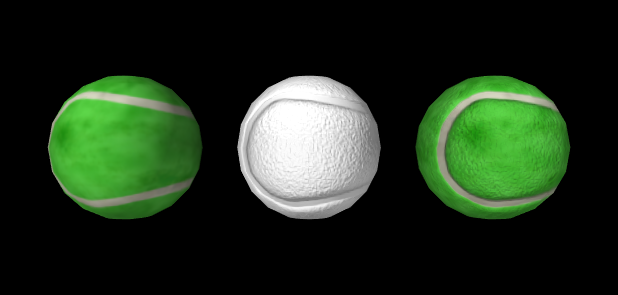
\includegraphics[]{images/sphericalMapping}
\else
 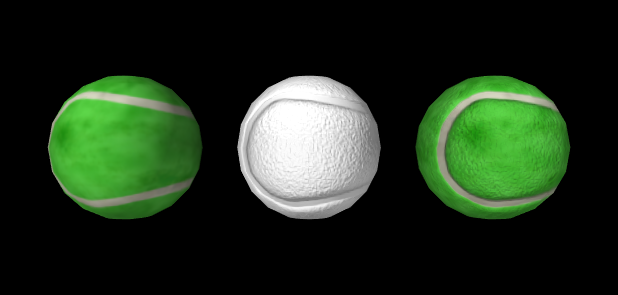
\includegraphics[width=4.5in]{images/sphericalMapping}
\fi
\end{center}
\caption{Color and bump mapping applied to spherical meshes. Left:
color mapping only. Middle: bump mapping only. Right: combined color
and bump mapping.}
\label{sphericalMapping:fig}
\end{figure}

\lstset{numbers=left}
\lstinputlisting{../../src/artisynth/demos/tutorial/SphericalTextureMapping.java}
\lstset{numbers=none}

The {\tt build()} method uses the internal method {\tt createBall()}
to generate three rigid bodies, each defined using a spherical mesh
that has been created with
\javamethodAlt{maspack.geometry.MeshFactory.createSphere(double,int,int,boolean)}%
{MeshFactory.createSphere()} with {\tt addTextureCoords} set to {\tt
true}.  The remainder of the {\tt build()} method sets up the render
properties and the texture mappings. Two texture mappings are defined:
a color mapping and bump mapping, based on the images {\tt
TennisBallColorMap.jpg} and {\tt TennisBallBumpMap.jpg} (Figure
\ref{mappingImages:fig}), both located in the subdirectory {\tt data}
relative to the demo source file.
\javamethod[maspack.util]{PathFinder.expand()} is used to determine
the full data folder name relative to the source directory.
For the bump map, it is important to set the {\sf scaling} property
to adjust the depth applitude to relative to the sphere radius.

\begin{figure}[ht]
\begin{center}
\begin{tabular}{c}
   \iflatexml
      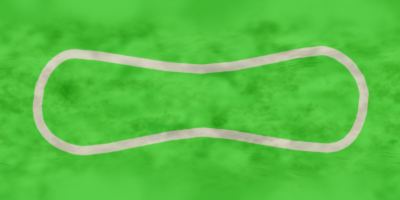
\includegraphics[]{images/TennisBallColorMap}\\
      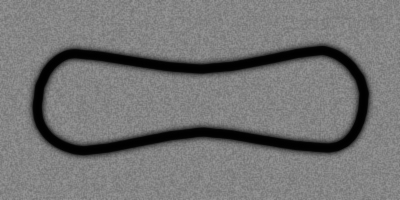
\includegraphics[]{images/TennisBallBumpMap}
   \else
      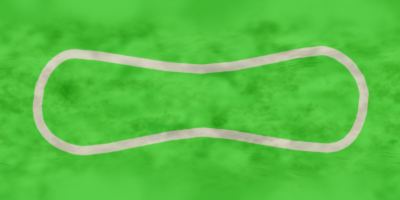
\includegraphics[width=3in]{images/TennisBallColorMap}\\
      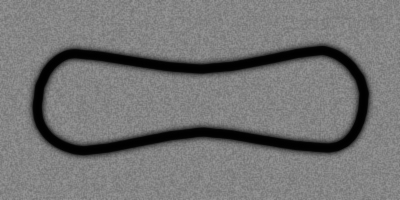
\includegraphics[width=3in]{images/TennisBallBumpMap}
   \fi
\end{tabular}
\end{center}
\caption{Color and bump map images used in the texture mapping example.
These map to spherical coordinates on the mesh.}
\label{mappingImages:fig}
\end{figure}

Color mapping is applied to balls 0 and 2, and bump mapping to balls 1
and 2. To illustrate setting mapping properities in an ancestor
component, the color mapping is arranged by setting the {\sf colorMap}
render property of the {\tt MechModel}, and then, as described above,
enabling color mapping within the individual balls.

To run this example in ArtiSynth, select {\sf All demos > tutorial >
SphericalTextureMapping} from the {\sf Models} menu. The model should
load and initially appear as in Figure
\ref{sphericalMapping:fig}. Note that if ArtiSynth is run with the
legacy OpenGL 2 viewer (commmand line option {\tt -GLVersion 2}), bump
mapping will not be supported and will not appear.

\section{Point-to-point muscles}
\label{PointToPointMuscles:sec}

Point-to-point muscles are a simple type of component in biomechanical
models that provide muscle-activated forces acting along a line
between two points. ArtiSynth provides this through
\javaclass[artisynth.core.mechmodels]{Muscle}, which is a subclass of
\javaclass[artisynth.core.mechmodels]{AxialSpring} that generates an
active muscle force in response to its {\tt excitation} property. The
excitation property can be set and queried using the methods
%
\begin{lstlisting}[]
   setExcitation (double a);
   double getExcitation();
\end{lstlisting}
%

\subsection{Muscle materials}
\label{sec:mechii:musclematerials}

As with {\tt AxialSpring}s, {\tt Muscle} components use an
\javaclass[artisynth.core.materials]{AxialMaterial} to compute the
applied force $f (l, \dot l, a)$ in response to the muscle's length
$l$, length velocity $\dot l$, and excitation signal $a$.  Usually the
force is the sum of a {\it passive} component plus an {\it active}
component that arises in response to the excitation signal.

The default {\tt AxialMaterial} for a {\tt Muscle} is
\javaclass[artisynth.core.materials]{SimpleAxialMuscle},
which is essentially an activated version of 
\javaclass[artisynth.core.materials]{LinearAxialMaterial}
and 
which computes a simple force according to
%
\begin{equation}
f(l, \dot l) = k (l-l_0) + d \dot l + m_f a
\end{equation}
%
where $k$ and $d$ are stiffness and damping terms, $a$ is the
excitation value, and $m_f$ is the maximum excitation force.
$k$, $d$ and $m_f$ are exposed through the properties {\tt
stiffness}, {\tt damping}, and {\tt maxForce}.

More complex muscle materials are typically used for biomechanical
modeling applications, generally with non-linear passive terms and
active terms that depend on the muscle length $l$.  Some of those
available in ArtiSynth include
\javaclass[artisynth.core.materials]{ConstantAxialMuscle},
\javaclass[artisynth.core.materials]{BlemkerAxialMuscle},
\javaclass[artisynth.core.materials]{PaiAxialMuscle}, and
\javaclass[artisynth.core.materials]{PeckAxialMuscle}.

% LATER: describe muscles in more detail

\subsection{Example: Muscle attached to a rigid body}
\label{SimpleMuscleExample:sec}

\begin{figure}[ht]
\begin{center}
\iflatexml
 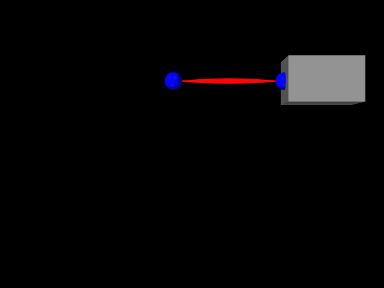
\includegraphics[]{images/SimpleMuscle}
\else
 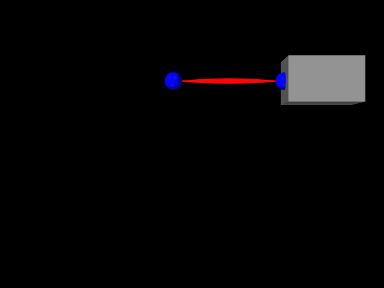
\includegraphics[width=3.75in]{images/SimpleMuscle}
\fi
\end{center}
\caption{SimpleMuscle model loaded into ArtiSynth.}
\label{SimpleMuscle:fig}
\end{figure}

A simple model showing a single muscle connected to a rigid
body is defined in
%
\begin{verbatim}
  artisynth.demos.tutorial.SimpleMuscle
\end{verbatim}
%

This model is identical to {\tt RigidBodySpring} described in Section
\ref{RigidBodySpringExample:sec}, except that the code to create
the spring is replaced with code to create a muscle
with a {\tt SimpleAxialMuscle} material:
%
\begin{lstlisting}[]
      // create the muscle:      
      muscle = new Muscle ("mus", /*restLength=*/0);
      muscle.setPoints (p1, mkr);
      muscle.setMaterial (
         new SimpleAxialMuscle (/*stiffness=*/20, /*damping=*/10, /*maxf=*/10));
\end{lstlisting}
%
Also, so that the muscle renders differently, the rendering style
for lines is set to {\tt SPINDLE} using the convenience method
%
\begin{lstlisting}[]
      RenderProps.setSpindleLines (muscle, 0.02, Color.RED);
\end{lstlisting}
%

To run this example in ArtiSynth, select {\sf All demos > tutorial >
SimpleMuscle} from the {\sf Models} menu. The model should load and
initially appear as in Figure \ref{SimpleMuscle:fig}.  Running the
model (Section \ref{LoadingAndRunning:sec}) will cause the box to fall
and sway under gravity. To see the effect of the {\tt excitation}
property, select the muscle in the viewer and then choose {\sf Edit
properties ...} from the right-click context menu.  This will open an
editing panel that allows the muscle's properties to be adjusted
interactively. Adjusting the {\tt excitation} property using the
adjacent slider will cause the muscle force to vary.

% LATER \subsection{Multi-point muscles}

% LATER \section{Mesh components}
%OPTIONAL 
% LATER \subsection{Fixed meshes}
% LATER \subsection{Simple mesh example}

% SimpleMesh

% LATER \subsection{Skinned meshes}
% LATER \subsection{Simple skinned mesh example}

% SimpleSkinnedMesh

\section{Collision Handling}
\label{sec:mechii:collisions}

Collision handling in ArtiSynth is implemented by a collision
handling mechanism build into {\tt MechModel}. Collisions are
disabled by default, but can be enabled between rigid and deformable
bodies (finite element models in particular), and more generally
between any body that implements the interface 
\javaclass[artisynth.core.mechmodels]{Collidable}.

It is important to understand that collison handling is both
computationally expensive and, due to it's discontinuous nature, less
accurate than other aspects of the simulation.  ArtiSynth therefore
provides a number of ways to selectively control collision handling
between different pairs of bodies.

%\subsection{Collidable bodies}

\subsection{Enabling collisions in code}

Collisions can be enabled as either a default behavior between all
bodies, a default behavior between certain {\it types} of
bodies, or a specific behavior between individual pairs of bodies.

The default collision behavior between all collidables can be
controlled using two equivalent methods:
%
\begin{lstlisting}[]
  setDefaultCollisionBehavior (enabled, mu);
  setDefaultCollisionBehavior (behavior);
\end{lstlisting}
%
where {\tt enabled} is {\tt true} or {\tt false} depending on whether
collisions are enabled, {\tt mu} is the coefficient of Coulomb (or
dry) friction, and {\tt behavior} is a
\javaclass[artisynth.core.mechmodels]{CollisionBehavior} object that
specifies both {\it enabled} and {\it mu}. The {\tt mu} value is
ignored if {\tt enabled} is {\tt false}.  In addition, collisions can
be controlled for specific {\it types} of collidables using
%
\begin{lstlisting}[]
  setDefaultCollisionBehavior (typeA, typeB, enabled, mu);
  setDefaultCollisionBehavior (typeA, typeB, behavior);
\end{lstlisting}
%
where {\tt typeA} and {\tt typeB} should be either {\tt
Collidable.RigidBody} or {\tt Collidable.Deformable}.  In addition,\\
{\tt Collidable.Deformable} can be paired with {\tt Collidable.Self} to
enable/disable self-collisions between deformable objects.
Self-collision is described in greater detail in Section
\ref{SelfCollision:sec}.

A call to one of the {\tt setDefaultCollisionBehavior()} methods will
override the effects of previous calls. So for instance, the code
sequence
%
\begin{lstlisting}[]
  setDefaultCollisionBehvaior (true, 0);
  setDefaultCollisionBehvaior (
    Collidable.Deformable, Collidable.RigidBody, false, 0);
  setDefaultCollisionBehavior (true, 0.2);
\end{lstlisting}
%
will initially enable collisions between all bodies with a friction
coefficient of 0, then {\it disable} collisions between deformable and
rigid bodies, and finally re-enable collisions between all bodies with
a friction coefficient of 0.2.

The default collision behavior between any pair of body types can
be queried using
%
\begin{lstlisting}[]
  CollisionBehavior getDefaultCollisionBehavior (typeA, typeB);
\end{lstlisting}
%

In addition to default behaviors, collisions between individual
collidables can be controlled and queried using
%
\begin{lstlisting}[]
  setCollisionBehavior (collidableA, collidableB, enabled, mu);
  setCollisionBehavior (collidableA, collidableB, behavior);
  getCollisionBehavior (collidableA, collidableB);
\end{lstlisting}
%
where {\tt collidableA} and {\tt collidableB} are individual
collidable components such as rigid bodies or FEM models.  Collision
behaviors specified by {\tt setCollisionBehavior()} {\it override} the
default collision behaviors, and are {\it not} invalidated by
subsequent calls to the {\tt setDefaultCollisionBehavior()} methods.
An overide collision behavior for a specific pair of collidables
can be removed by
%
\begin{lstlisting}[]
  clearCollisionBehavior (collidableA, collidableB);
\end{lstlisting}
%
and {\it all} override behaviors in a {\tt MechModel} can
be removed by 
%
\begin{lstlisting}[]
  clearCollisionBehaviors ();
\end{lstlisting}
%

\begin{sideblock}
Note: It is usually necessary to ensure that collisions are {\it disabled}
between adjacent bodies connected by joints, since otherwise these
would be forced into a state of permanent collision.
\end{sideblock}

\subsection{Example: Collision with a plane}
\label{JointedCollide:sec}

\begin{figure}[ht]
\begin{center}
\iflatexml
 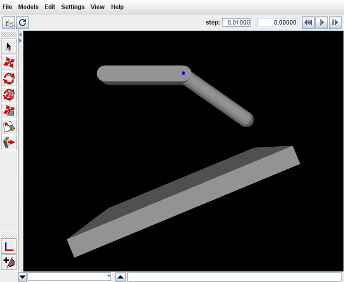
\includegraphics[]{images/JointedCollide}
\else
 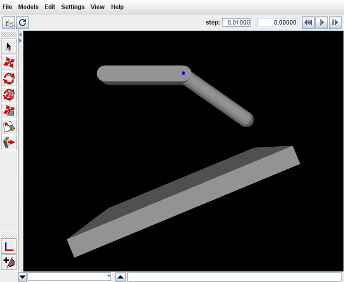
\includegraphics[width=3.75in]{images/JointedCollide}
\fi
\end{center}
\caption{JointedCollide model loaded into ArtiSynth.}
\label{JointedCollide:fig}
\end{figure}

A simple model illustrating collision between two jointed rigid bodies
and a plane is defined in
%
\begin{verbatim}
  artisynth.demos.tutorial.JointedCollide
\end{verbatim}
%

This model is simply a subclass of {\tt RigidBodyJoint} that
overrides the {\tt build()} method 
to add an inclined plane and enable collisions between it and
the two connected bodies:
%
\lstset{numbers=left}
\begin{lstlisting}[]
   public void build (String[] args) {

      super.build (args);

      bodyB.setDynamic (true);  // allow bodyB to fall freely

      // create and add the inclined plane
      RigidBody base = RigidBody.createBox ("base", 25, 25, 2, 0.2);
      base.setPose (new RigidTransform3d (5, 0, 0, 0, 1, 0, -Math.PI/8));
      base.setDynamic (false);
      mech.addRigidBody (base);

      // turn on collisions
      mech.setDefaultCollisionBehavior (true, 0.20);
      mech.setCollisionBehavior (bodyA, bodyB, false);
   }
\end{lstlisting}
\lstset{numbers=none}

The superclass {\tt build()} method called at line 3 creates
everything contained in {\tt RigidBodyJoint}. The remaining code then
alters that model: {\tt bodyB} is set to be dynamic (line 5) so that
it will fall freely, and an inclined plane is created from a thin box
that is translated and rotated and then set to be be non-dynamic
(lines 8-11).  Finally, collisions are enabled by setting the default
collision behavior (line 14), and then specifically disabling
collisions between {\tt bodyA} and {\tt bodyB} (line 15). As indicated
above, the latter step is necessary because the joint would otherwise
keep the two bodies in a permanent state of collision.

To run this example in ArtiSynth, select {\sf All demos > tutorial >
JointedCollide} from the {\sf Models} menu. The model should load and
initially appear as in Figure \ref{JointedCollide:fig}.  Running
the model (Section \ref{LoadingAndRunning:sec}) will
cause the jointed assembly to collide with and slide off the inclined
plane.


\subsection{Self-collision and collidable hierarchies}
\label{SelfCollision:sec}

At present, {\tt ArtiSynth} does not support the detection or handling
of self-collision within single meshes. However, self-collision can
still be effected by allowing a collidable to have multiple
{\it sub-collidables} and then enabling collisions between some or all of
these.

Any descendant component of a
\javaclass[artisynth.core.mechmodels]{Collidable} component A which is
itself {\tt Collidable} is considered to be a sub-collidable of A.
Certain types of components maintain sub-collidables by default.  For
example, some components (such as finite element models; Section
\ref{FEMModels:sec}) maintain a list of meshes in a child component
list named {\tt meshes}; these can be used to implement self-collision
as described below.

\begin{sideblock}
Note: A collidable does not need to be an immediate child component
of a collidable A in order to be a sub-collidable of A;
it need only be a descendent of A. 
\end{sideblock}

\begin{figure}[ht]
\begin{center}
 \iflatexml
   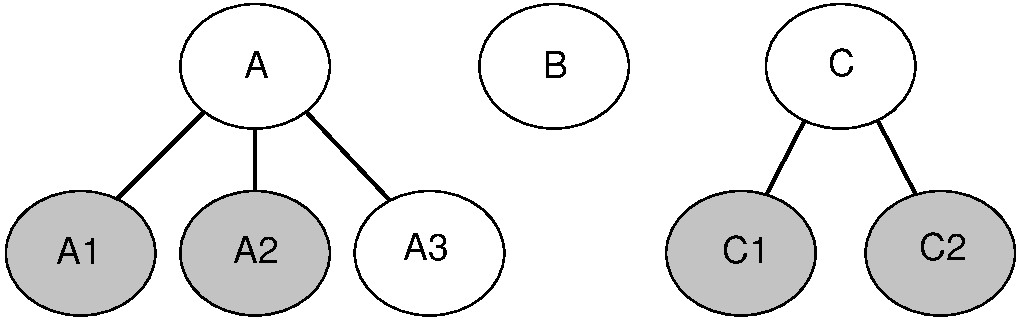
\includegraphics[width=5in]{images/CollidableGroups}
 \else
   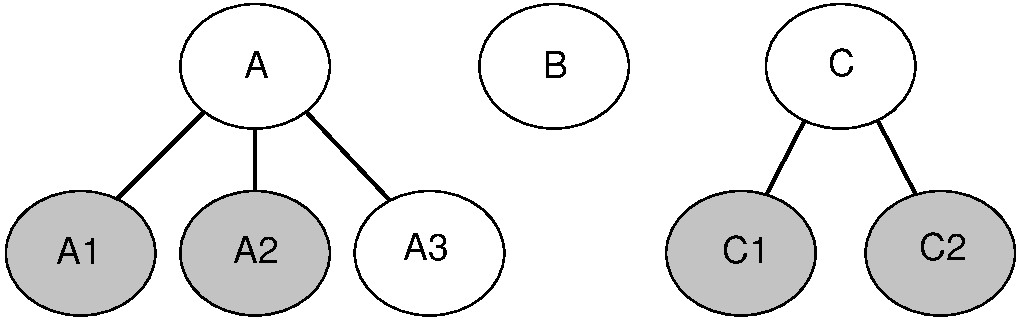
\includegraphics[width=5in]{images/CollidableGroups.idr}
 \fi
\end{center}
\caption{A collection of collidable components, where A possesses
sub-collidables A1, A2, and A3, B is solitary, and C possesses
sub-collidables C1 and C2. Internal collisions are enabled among those
sub-collidables which are shaded gray.}
\label{CollidableGroups:fig}
\end{figure}

In general, an ArtiSynth model will contain a collection of
collidables, some of which posses sub-collidables and others which are
solitary (Figure \ref{CollidableGroups:fig}).  Within a collection of
collidables:

\begin{itemize}

\item Actual collisions happen only between leaf collidables; ancestor
collidables are used only for grouping purposes.

\item By default, the sub-collidables of a component A will only
collide among themselves if self-collision is specified for A (via
either a default or override collision behavior). If self-collision is
specified for A, then collisions may occur only among those
sub-collidables for which {\it internal} collisions are enabled.
Internal collisions are enabled for a collidable if its {\tt
collidable} property (Section \ref{collidability:sec}) is set to
either {\tt ALL} or {\tt INTERNAL}.

\item Self-collision is also only possible among the sub-collidables
of A if A is itself deformable; i.e., its
\javamethod[artisynth.core.mechmodels.Collidable]{isDeformable()}
method returns {\tt true}.

\item Sub-collidables may collide with collidables outside their
hierarchy if their {\tt collidable} property is set to either {\tt
ALL} or {\tt EXTERNAL}.

\item Collision among specific pairs of sub-collidables may also be
explicitly enabled or disabled with an override behavior set using one
of the {\tt setCollisionBehavior()} methods.

\item Specifying a collision behavior among two collidables A and B
which are {\it not} within the same hierarchy will cause that behavior
to be specified among all sub-collidables of A and B whose {\tt
collidable} property enables the collision.

\end{itemize}

This is best illustrated with some examples. Refer to Figure
\ref{CollidableGroups:fig}, assume that components A, B and C are
deformable, and that self-collision is allowed among those
sub-collidables which are shaded gray (A1 and A2 for A, B1 and B2 for
B). Then:
%
\begin{lstlisting}[]
   // Set default collision among deformable components with friction = 0.2:
   setDefaultCollisionBehavior (
      Collidable.DEFORMABLE, Collidable.DEFORMABLE, true, 0.2);
   // Collisions are now enabled between A1, A2, and A3 and each of B, C1, and
   // C2, and between B and C1 and C2, but not among A1, A2, and A3 or C1 and C2.

   // Enable self-collision between A1 and A2 and B1 and B2 with friction = 0:
   setDefaultCollisionBehavior (Collidable.DEFORMABLE, Collidable.SELF, true, 0);
    
   // Specifically disable collision between B and A3:
   setCollisionBehavior (B, A3, false);

   // Specifically enable collision between A3 and C with friction = 0.3:
   setCollisionBehavior (A3, C, true, 0.3);
   // This behavior will be applied between A3 and each of C1 and C2.

   // Disable self-collision within A:
   setCollisionBehavior (A, A, false);
   // This will disable all self-collisions among A1, A2 and A3.
\end{lstlisting}
%

\subsection{Collidability}
\label{collidability:sec}

Each collidable component maintains a {\tt collidable} property
(which can be queried using
\javamethod[artisynth.core.mechmodels.Collidable]{getCollidable()})
which specifically enables or disables the ability of that collidable
to collide with other collidables.

The {\tt collidable} property value is of the enumerated type
\javaclass[artisynth.core.mechmodels]{Collidable\$Collidability}, which
has four possible settings:

\begin{description}

\item[OFF]\mbox{}

All collisions disabled: the collidable will not collide with
anything.

\item[INTERNAL]\mbox{}

Internal (self) collisions enabled: the collidable may only collide
with other Collidables with which it shares a common ancestor.

\item[EXTERNAL]\mbox{}

External collisions enabled: the collidable may only collide with
other Collidables with which it does {\it not} share a common
ancestor.

\item[ALL]\mbox{}

All collisions (both self and external) enabled: the collidable may
collide with any other Collidable.

\end{description}

Note that collidability only {\it enables} collisions.  In order for
collisions to actually occur between two collidables, a default or
override collision behavior must also be specified for them in the
MechModel.

\subsection{Implementation and limitations}

The ArtiSynth collision mechanism works by finding intersections
between the surface meshes of each collidable object.  These surface
meshes must (at present) be triangular, closed, and manifold.
A bounding-box 
hierarchy is used to determine if any two surfaces meshes
intersect. If they do, then a tracing algorithm
is used to compute all the intersection contours
between the two meshes as shown in Figure~\ref{Collision:fig}.

\begin{figure}[ht]
\begin{center}
        \begin{tabular}{ccc}
        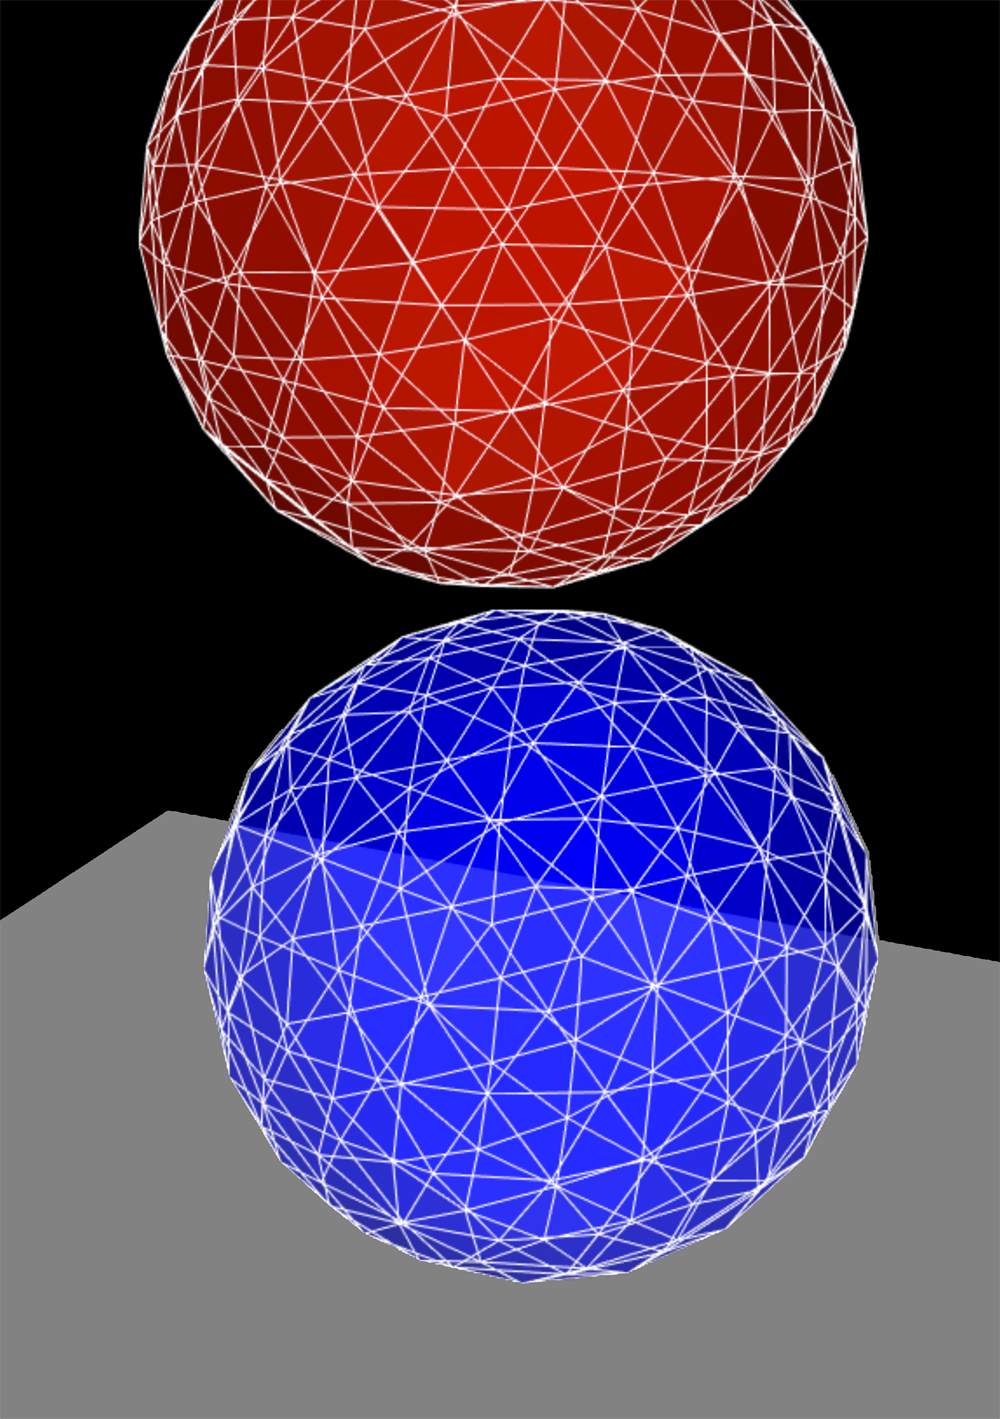
\includegraphics[width=0.31\textwidth]{images/femCollide1} &
        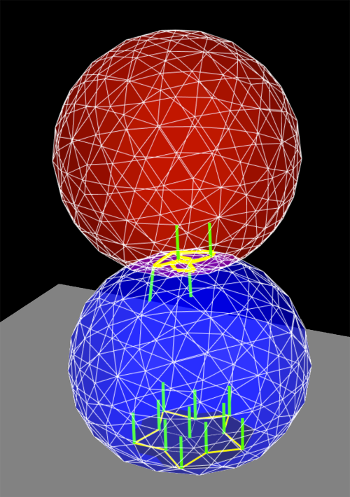
\includegraphics[width=0.31\textwidth]{images/femCollide2} &
        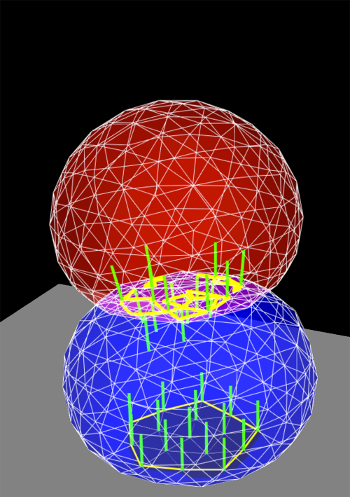
\includegraphics[width=0.31\textwidth]{images/femCollide3}\\
%       \end{tabular}
%       \begin{tabular}{p{1.2cm}p{3.5cm}p{3.5cm}p{3.5cm}} 
         \large  $\mathrm{t}=0$s & \large $\mathrm{t}=0.25$s & \large $\mathrm{t}=0.5$s         
        \end{tabular}
\end{center}
\caption{Time sequence of contact handling between two deformable models 
falling under gravity, 
showing the intersection contours
(yellow) and the contact normals (green lines).}
\label{Collision:fig}
\end{figure}

% XXX -useAjlCollision and contours?

Determining the intersection contour allows us to create a set of
constraints for correcting the interpenetration and preventing
interpenetrating velocities.  For rigid bodies, this is done by
fitting a plane to each contour, projecting the contour onto this
plane, and then sampling the vertices of the projection's 2D convex
hull to create individual contact points, with the contact normal set
from the normal of the plane. For deformable FEM models, the
intersection contour is used to locate all the interpenetrating nodes,
and then collision constraints are established between each node and
the nearest triangular face of the opposing surface.

Because ArtiSynth currently uses static collision detection, it is
possible for objects that are fast enough or thin enough to completely
pass through each other in one simulation step. This means that for
thin objects, it is important to keep the step size small enough to
prevent such undetected interpenetration.

ArtiSynth also uses a ``box'' friction approximation
\cite{Lacoursiere07} to compute dry friction, instead of the
polyhedralized friction cones common in the multibody dynamics
literature \cite{AnitescuPotra2002,PotraEtAlTrapezoidal2006}.  This
allows for a less expensive and more robust computation at the expense
of some accuracy.

Another issue is that ArtiSynth's attempt to separate colliding bodies
at the end of each time step may cause a jittering behavior around the
colliding area, as the surface collides, separates, and re-collides.
This can usually be stabilized by maintaining a certain
interpenetration distance during contact. This distance is controlled
by the {\tt MechModel} property {\tt penetrationTol}.  ArtiSynth
attempts to compute a suitable default value for this property, but
for some applications it may be necessary to control the value
explicitly using the {\tt MechModel} methods
%
\begin{lstlisting}[]
   setInterpenetrationTol (double dist);
   double getInterpenetrationTol();
\end{lstlisting}
%

Other aspects of collision handling can be adjusted by directly
setting properties of the {\tt MechModel}'s collision manager, which
can be accessed graphically via the navigation panel, or in code using
\javamethod*[artisynth.core.mechmodels.MechModel]{getCollisionManager()}.

One of these properties is {\tt collisionPointTol}, which for
collisions between rigid bodies specifies a minimum distance between
contact points and therefore can be used to reduce the number of
contact constraints and improve computation time.

\subsection{Contact rendering}

The {\tt MechModel}'s collision manager component contains render
properties that can be used to render the contact points, normals, and
mesh intersection contours associated with contact.

By default, contact and contour rendering is disabled. To enable it,
one can use the following code fragment:
%
\begin{verbatim}
  RenderProps.setVisible (mechModel.getCollisionManager(), true);
\end{verbatim}
%
The following render properties are used:

\begin{description}

\item[lineStyle] \mbox{}
Style of the line used for rendering the contact normals

\item[lineWidth] \mbox{}
Width (in pixels) of the contact normal if the {\tt Line} line style is used

\item[lineRadius] \mbox{}
Radius of the contact normal if a solid line style is used

\item[lineColor] \mbox{}
Color of the contact normal

\item[edgeWidth] \mbox{}
Width (in pixels) of the line used to render the contour

\item[edgeColor] \mbox{}
Color of the contour

\end{description}

These properties can be set in the same way as the visibility, using
the {\tt RenderProps} methods presented in Section
\ref{SettingRenderProperties:sec}:

\begin{lstlisting}[]
  Renderable colManager = mechModel.getCollisionManager();
  RenderProps.setEdgeWidth (col, 2);
  RenderProps.setEdgeColor (col, Color.Red);
\end{lstlisting}

To access these properties on a read-only basis, one can do
  
\begin{lstlisting}[]
  RenderProps props = mechModel.getCollisionManager().getRenderProps();
\end{lstlisting}

Finally, to set the length of the rendered contact normals, set the
{\tt contactNormalLen} property in collision manager. Since contact
normals have no preferred direction, it may be necessary to use a
negative length value in order to visualize them properly.

A simple model showing a contact rendering is defined in
%
\begin{verbatim}
  artisynth.demos.tutorial.BallPlateCollide
\end{verbatim}
%
and the complete source code is shown below:
%
\lstset{numbers=left}
\lstinputlisting{../../src/artisynth/demos/tutorial/BallPlateCollide.java}
\lstset{numbers=none}

To run this example in ArtiSynth, select {\sf All demos > tutorial >
BallPlateCollide} from the {\sf Models} menu. When run, the ball
will collide with the plate and the contact normals and collision 
contours with be draw and shown in Figure \ref{BallPlateCollide:fig}.

\begin{figure}[ht]
\begin{center}
\iflatexml
 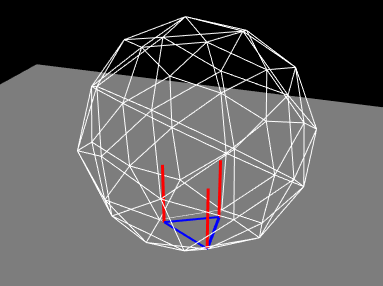
\includegraphics[]{images/BallPlateCollide}
\else
 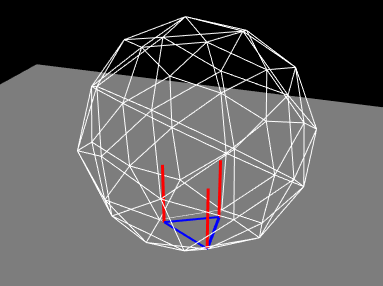
\includegraphics[width=3.75in]{images/BallPlateCollide}
\fi
\end{center}
\caption{BallPlateCollide showing contact normals (red) and collision contour
(blue) of the ball colliding with the plate.}
\label{BallPlateCollide:fig}
\end{figure}

\section{Transforming geometry}
\label{TransformingGeometry:sec}

Certain ArtiSynth components, including {\tt MechModel}, implement the
interface \javaclass[artisynth.core.modelbase]{TransformableGeometry},
which allows the geometric transformation of the component's
attributes (such as meshes, points, frame locations, etc.), along with
its descendant components. The interface provides the method
%
\begin{lstlisting}[]
   public void transformGeometry (AffineTransform3dBase X);
\end{lstlisting}
%
where {\tt X} is an \javaclass[maspack.matrix]{AffineTransform3dBase}
that may be either a \javaclass[maspack.matrix]{RigidTransform3d} or a
more general \javaclass[maspack.matrix]{AffineTransform3d} (Section
\ref{RigidTransform3d:sec}).

\javamethodAlt{artisynth.core.modelbase.TransformableGeometry.transformGeometry()}%
{transformGeometry(X)}
can be used to translate, rotate, shear or scale components. It
can be applied to an entire model or individual components. Unlike
\javamethod*[artisynth.core.util.ScalableUnits]{scaleDistance()}, it
actually changes the physical geometry and so may change the
simulation behaviour. For example, applying {\tt transformGeometry()}
to a \javaclass[artisynth.core.mechmodels]{RigidBody} will cause the
shape of its mesh to change, which will change its mass if its {\sf
inertiaDensity} property is set to {\sf Density}.
Figure \ref{RigidAndAffineTransforms:fig} shows a simplified
illustration of both rigid and affine transformations being applied to
a model.

\begin{figure}[ht]
\begin{center}
   \begin{tabular}{ccc}
   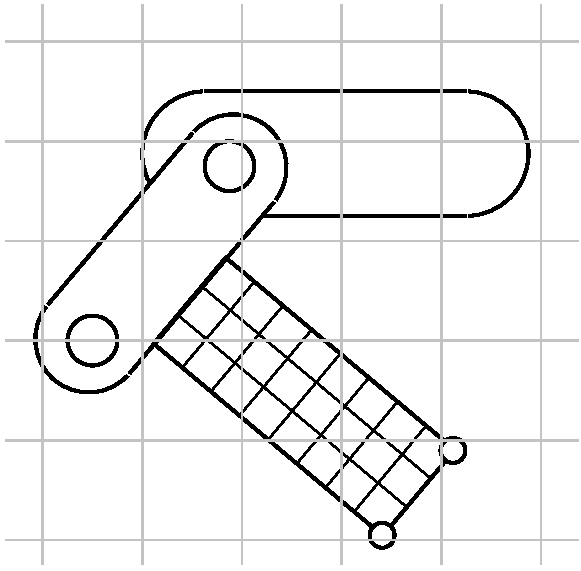
\includegraphics[width=0.27\textwidth]{images/tgenModel} &
   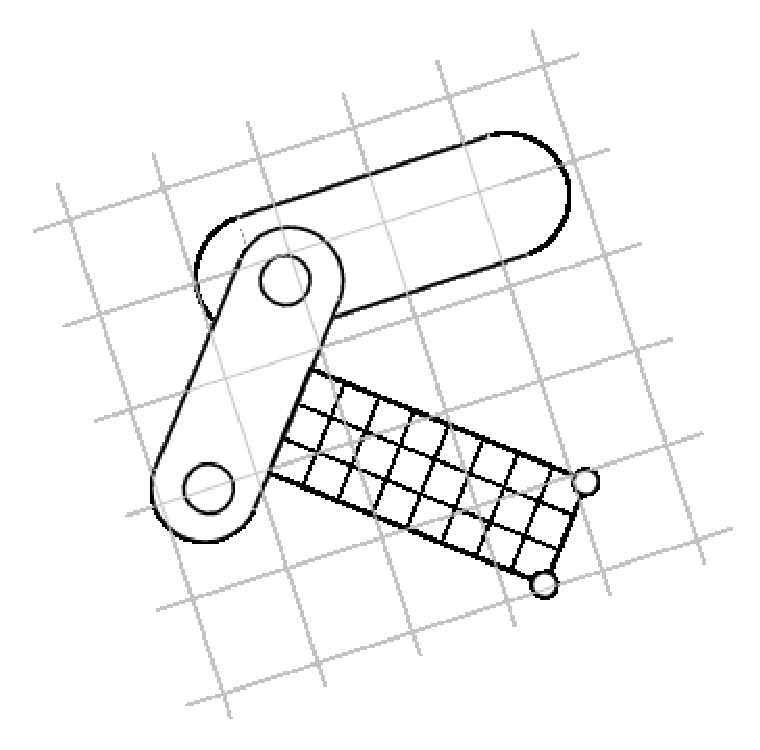
\includegraphics[width=0.34\textwidth]{images/tgenModelRigid} &
   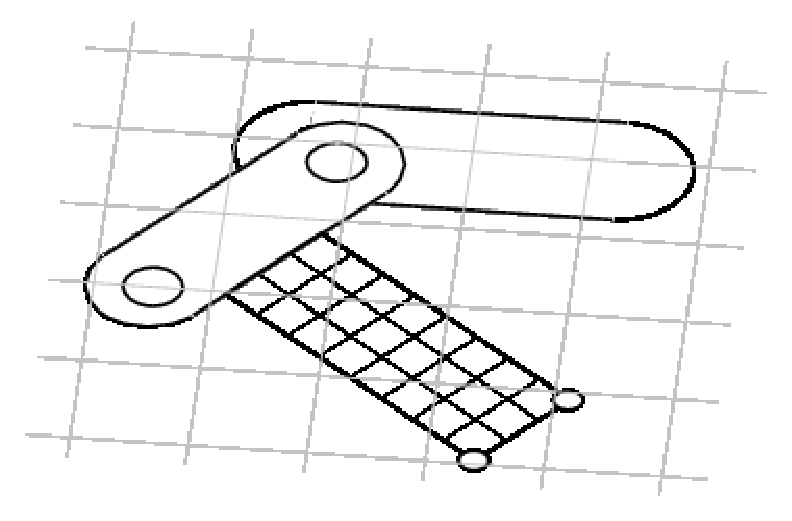
\includegraphics[width=0.34\textwidth]{images/tgenModelAffine}
   \end{tabular}
\end{center}
\caption{Simple illustration of a model (left) undergoing a rigid
transformation (middle) and an affine transformation (right).}
\label{RigidAndAffineTransforms:fig}
\end{figure}

The example below shows how to apply a transformation to a model in
code. In it, a {\tt MechModel} is first scaled by the factors 1.5, 2,
and 3 along the x, y, and z axes, and then flipped upside down using a
{\tt RigidTransform3d} that rotates it by 180 degrees about the x
axis:
%
\begin{lstlisting}[]
   MechModel mech;

   ... build mech model ...

   AffineTransform3d X = new AffineTransform3d();
   X.applyScaling (1.5, 2, 3);
   mech.transformGeometry (X);
   
   RigidTransform3d T = 
      new RigidTransform3d (/*x,y,z=*/0, 0, 0, /*r,p,y=*/0, 0, Math.PI);
   mech.transformGeomerty (T);
\end{lstlisting}
%

\subsection{Nonlinear transformations}

The \javaclass[artisynth.core.modelbase]{TransformableGeometry}
interface also supports general, non-linear geometric transforms.
This can be done using a
\javaclass[maspack.geometry]{GeometryTransformer}, which is an
abstract class for performing general transformations.  To apply such
a transformation to a component, one can create and initialize an appropriate
subclass of {\tt
GeometryTransformer} to perform the desired transformation, and
then apply it using the static {\tt transform} method of the utility class 
\javaclass[artisynth.core.modelbase]{TransformGeometryContext}:
%
\begin{lstlisting}[]
  ModelComponent comp;     // component to be transformed
  GeometryTransformer gtr; // transformer to do the transforming

  ... instantiate and initialize the transformer ...

  TransformGeometryContext.transform (comp, gtr, /*flags=*/0);
\end{lstlisting}
%

At present, the following subclasses of {\tt GeometryTransformer} are
available:

\begin{description}

\item[\protect{\javaclass[maspack.geometry]{RigidTransformer}}]\mbox{}

Implements rigid 3D transformations.

\item[\protect{\javaclass[maspack.geometry]{AffineTransformer}}]\mbox{}

Implements affine 3D transformations.

\item[\protect{\javaclass[artisynth.core.femmodels]{FemGeometryTransformer}}]\mbox{}

Implements a general transformation, using the deformation field
induced by a finite element model. 

\end{description}

\javaclass[artisynth.core.modelbase]{TransformGeometryContext} also
supplies the following convenience methods to apply transformations to
components or collections of components:
%
\begin{lstlisting}[]
    void transform (Iterable<TransformableGeometry>, GeometryTransformer, int);
    void transform (TransformableGeometry[], GeometryTransformer, int);

    void transform (TransformableGeometry, AffineTransform3dBase, int);
    void transform (Iterable<TransformableGeometry>, AffineTransform3dBase, int);
    void transform (TransformableGeometry[], AffineTransform3dBase, int);
\end{lstlisting}
%
The last three of these methods create an instance of either
\javaclass[maspack.geometry]{RigidTransformer} or
\javaclass[maspack.geometry]{AffineTransformer} for the supplied
\javaclass[maspack.matrix]{AffineTransform3dBase}. In fact, most
{\tt TransformableGeometry} components implement their
\javamethodAlt{artisynth.core.modelbase.TransformableGeometry.transformGeometry()}%
{transformGeometry(X)} method as follows:
%
\begin{lstlisting}[]
   public void transformGeometry (AffineTransform3dBase X) {
      TransformGeometryContext.transform (this, X, 0);
   }
\end{lstlisting}
%

The \javaclass[artisynth.core.femmodels]{FemGeometryTransformer}
class is derived from the
class \javaclass[maspack.geometry]{DeformationTransformer}, which uses
the single method
\javaclass[maspack.geometry.DeformationTransformer]{getDeformation()} to
obtain deformation field information at a specified reference postion:
%
\begin{lstlisting}[]
    void getDeformation (Vector3d p, Matrix3d F, Vector3d r)
\end{lstlisting}
%
If the deformation field is described by $\x' = f(\x)$, then
for a given reference position $\r$ (in undeformed coordinates),
this method should return the deformed position $\p = f(\r)$
and the deformation gradient
%
\begin{equation}
\F \equiv \frac{\partial f}{\partial \x}
\end{equation}
%
evaluated at $\r$. 

\javaclass[artisynth.core.femmodels]{FemGeometryTransformer} obtains
$f(\x)$ and $\F$ from a
\javaclass[artisynth.core.femmodels]{FemModel3d} (see Section
\ref{FEMModels:sec}) whose elemental rest positions enclose the
components to be transformed, using the fact that a finite element
model creates an implied piecewise-smooth deformation field as it
deviates from its rest position. For each reference point $\r$ needed
by the transformation process, {\tt FemGeometryTransformer} finds the
FEM element whose rest volume encloses $\r$, and then uses the
corresponding shape function coordinates to compute $f(\x)$ and $\F$
from the element's deformation. If the FEM model does {\it not}
enclose $\r$, the nearest element is used to determine the shape
function coordinates (however, this calculation becomes less accurate and
meaningful the farther $\r$ is from the FEM model). Transformations based
on FEM models are further illustrated in Section
\ref{FemModelDeformer:sec}, and by Figure
\ref{JointedCollideDeformation:fig}. Full details on ArtiSynth finite
element models are given in Section \ref{FEMModels:sec}.

Besides FEM models, there are numerous other ways to create
deformation fields, such as radial basis functions, thin plate
splines, etc. Some of these may be more appropriate for a particular
application and can provide deformations that are globally smooth (as
opposed to piecewise smooth).  It should be relatively easy for an
application to create its own subclass of {\tt DeformationTransformer}
to implement the deformation of choice by overriding the single
\javaclass[maspack.geometry.DeformationTransformer]{getDeformation()}
method.

\subsection{Example: the FemModelDeformer class}
\label{FemModelDeformer:sec}

An FEM-based geometric transformation of a {\tt MechModel} is
facilitated by the class
\javaclass[artisynth.core.workspace]{FemModelDeformer}, which one can
add to an existing {\tt RootModel} to transform the geometry of a {\tt
MechModel} already located within that {\tt RootModel}.  {\tt
FemModelDeformer} subclasses
\javaclass[artisynth.core.femmodels]{FemModel3d} to include a
\javaclass[artisynth.core.femmodels]{FemGeometryTransformer}, and
provides some utility methods to support the transformation process.

A {\tt FemModelDeformer} can be added to a {\tt RootModel} by adding
the following code fragment to the end of the {\tt build()} method:
%
\begin{lstlisting}[]
   public void build (String[] args) {

      ... build the model ...

      FemModelDeformer deformer =
         new FemModelDeformer ("deformer", this, /*maxn=*/10);
      addModel (deformer);
      // add a control panel (this is optional)
      addControlPanel (deformer.createControlPanel());  
   }
\end{lstlisting}
%
When the deformer is created, its constructor searches the specified
{\tt RootModel} to locate the first top-level {\tt MechModel}. It then
creates a hexahedral FEM grid around this model, with {\tt maxn} specifying
the number of cells along the maximum dimension. Material and
mass properties of the model are computed automatically from the
underlying {\tt MechModel} dimensions (but can be altered if necessary after
construction). When added to the {\tt RootModel},
the deformer becomes another top-level model that can be deformed
independently of the {\tt MechModel} to create the required
deformation field, as described below. It also supplies application-defined
menu items that appear under the {\sf Application} menu in the ArtiSynth
menu bar (see Section \ref{MenuItems:sec}). 
The deformer's {\tt createControlPanel()} can also be used
to create a {\tt ControlPanel} (Section \ref{ControlPanels:sec}) that
controls the visiblity of the FEM model and the dynamic behavior of
both it and the {\tt MechModel}.

An example is defined in 
%
\begin{verbatim}
  artisynth.demos.tutorial.DeformedJointedCollide
\end{verbatim}
%
where the {\tt JointedCollide} example of Section
\ref{JointedCollide:sec} is extended to include a 
{\tt FemModelDeformer} using the code described above.

\begin{figure}[ht]
\begin{center}
\iflatexml
 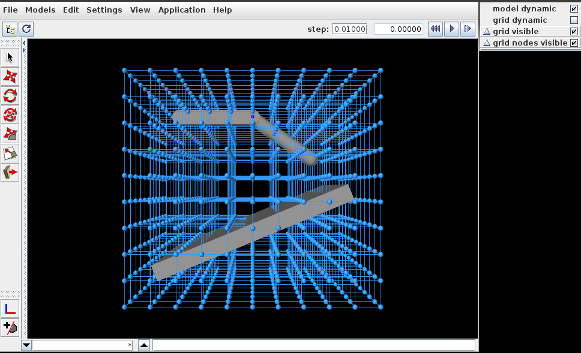
\includegraphics[]{images/DeformedJointedCollide}
\else
 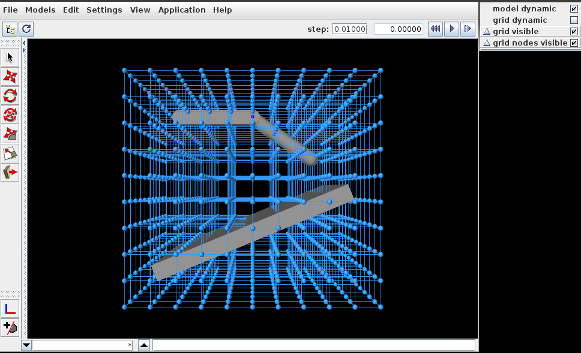
\includegraphics[width=5in]{images/DeformedJointedCollide}
\fi
\end{center}
\caption{The DeformedJointedCollide example initially loaded
into ArtiSynth.}
\label{DeformedJointedCollide:fig}
\end{figure}

To load this example in ArtiSynth, select {\sf All demos > tutorial >
DeformedJointedCollide} from the {\sf Models} menu. The model should load and
initially appear as in Figure \ref{DeformedJointedCollide:fig}, where
the control panel appears on the right.

The underlying {\tt MechModel} (or "model") can now be
transformed by first deforming the FEM model (or "grid") and
then using the resulting deformation field to effect the
transformation:

\begin{enumerate}

\item Make the model non-dynamic and the grid dynamic by unchecking
{\sf model dynamic} and checking {\sf grid dynamic} in the control
panel. This means that when simulation is run, the model will be inert
while the grid will respond physically.

\item Deform the grid using simulation. One easy way to do this is to
fix certain nodes, generally on or near the grid boundary, and then
move some of these using the translation or transrotator
tool while simulation is running. To fix a set of nodes, select
them in the viewer, choose {\sf Edit properties ...} from the
right-click context menu, and then uncheck their {\sf dynamic} property.
To easily select a large number of nodes without also selecting
model components or grid elements, one can specify {\tt FemNode}
in the selection filter widget. (See the sections
``Manipulation Tools'' and ``Selection filering'' in the
\href{\artisynthDocBase/html/uiguide/uiguide.html}{ArtiSynth User Interface Guide}.)

\item After the grid has been deformed, choose {\sf deform} from the
{\sf Application} menu in the ArtiSynth toolbar to transform the model.
Afterwards, the transformation can be undone by choosing {\sf undo},
and the grid can be reset by choosing {\sf reset grid}.

\item To run the deformed model after the transformation, it should
again be made dynamic by checking {\sf model dynamic} in the control
panel.  The itself grid can be made non-dynamic, and it and/or its
nodes can be made invisible by unchecking {\sf grid visible} and/or
{\sf grid nodes visible} in the control panel.

\end{enumerate}

The result of a possible deformation is shown in Figure
\ref{JointedCollideDeformation:fig}.

\begin{figure}[ht]
\begin{center}
  \begin{tabular}{cc}
  \iflatexml
    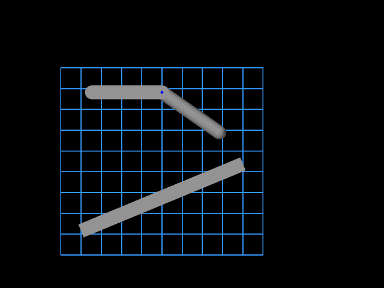
\includegraphics[]{images/DeformedJointedCollideBefore}&
    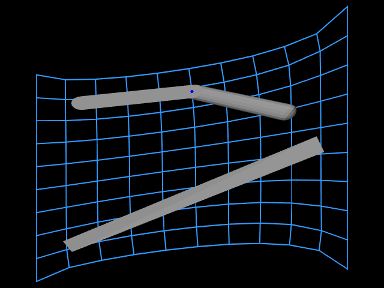
\includegraphics[]{images/DeformedJointedCollideAfter}
  \else
    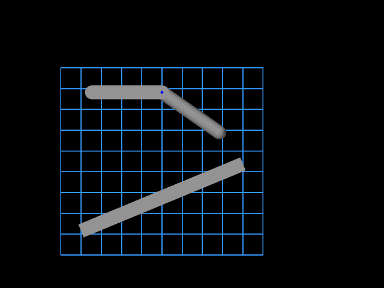
\includegraphics[width=0.45\textwidth]{images/DeformedJointedCollideBefore}&
    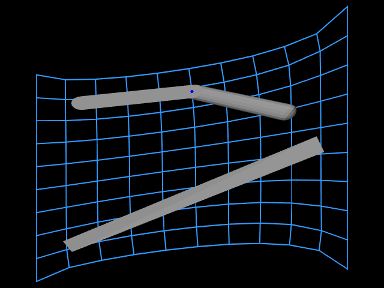
\includegraphics[width=0.45\textwidth]{images/DeformedJointedCollideAfter}
  \fi
  \end{tabular}
\end{center}
\caption{Deformation achieved in DeformedJointedCollide,
showing both the model and grid (using an orthographic view)
before and after the deformation.}
\label{JointedCollideDeformation:fig}
\end{figure}

\begin{sideblock}
Note: {\tt FemModelDeformer} is not intended to provide a general
purpose solution to non-linear geometric transformations. Rather, it
is mainly intended to illustrate the capabilities of
\javaclass[maspack.geometry]{GeometryTransformer} and the
\javaclass[artisynth.core.modelbase]{TransformableGeometry} interface.
\end{sideblock}

\subsection{Implementation and behavior}

As indicated above, the management of transforming the geometry for one
or more components is handled by the
\javaclass[artisynth.core.modelbase]{TransformGeometryContext} class.
The transform operations themselves are carried out by this class's
\javamethod[artisynth.core.modelbase.TransformGeometryContext]{apply()} 
method, which (a) assembles all the components that need
to be transformed, (b) performs the actual transform operations,
(c) invokes any required updating actions on other components,
and finally (d) notifies parent components of the change using
a \javaclass[artisynth.core.modelbase]{GeometryChangeEvent}.

To support this, ArtiSynth components which implement
\javaclass[artisynth.core.modelbase]{TransformableGeometry}
must also supply the methods
%
\begin{lstlisting}[]
   public void addTransformableDependencies (
      TransformGeometryContext context, int flags);

   public void transformGeometry (
      GeometryTransformer gtr, TransformGeometryContext context, int flags);
\end{lstlisting}
%
The first method,
\javamethodAlt{%
artisynth.core.modelbase.TransformableGeometry.addTransformableDependencies()}%
{addTransformableDependencies(context,flags)}, 
is called in step (a) to add to the context any additional components
which should be transformed along with this component. This includes
any descendants which should be transformed, since the
transformation of these should not generally be done within {\tt
transformGeometry(gtr,context,flags)}.

The second method, 
\javamethodAlt{%
artisynth.core.modelbase.TransformableGeometry.transformGeometry(,,)}%
{transformGeometry(gtr,context,flags)}, is
called in step (b) to perform the actual transformation on this
component.  It should use the supplied geometry transformer {\tt gtr}
to transform its attributes, as well as {\tt context} to query what
other components are also being transformed and to request
any needed updating actions to be called in step (c).  The {\tt flags} argument
specifies conditions associated with the transformation, which at the
moment may currently include:

\begin{description}

\item[TG\_SIMULATING]\mbox{}

The system is currently simulating, and therefore it may not be
desirable to transform all attributes;

\item[TG\_ARTICULATED]\mbox{}

Rigid body articulation constraints should
be enforced as the transform proceeds.

\end{description}

Full details for all this are given in the documentation for
\javaclass[artisynth.core.modelbase]{TransformGeometryContext}.

The transforming behavior of a component is up to its implementing
method, but the following rules are generally observed:

\begin{enumerate}

\item Transformable descendents are also transformed, by using {\tt
addTransformableDependencies()} to add them to the context as described
above;

\item When the nodes of an FEM model (Section \ref{FEMModels:sec}) are
transformed, the rest positions are also transformed if the system is
not simulating (i.e., if the {\tt TG\_SIMULATING} flag is not set).
This also causes the mass of the adjacent nodes to be recomputed from
the densities of the adjacent elements;

\item When dynamic components are transformed, any attachments and
constraints associated with them are updated appropriately, but only
if the system is not simulating. Non-transforming dynamic components
that are attached to transforming components as slaves are generally
updated so as to follow the transforming components to which they are
attached.

\end{enumerate}

\subsection{Use in model registration}

Transforming model geometry can obviously be used as part of the
process of creating subject-specific biomechanical and anatomical
models. However, registration will generally require more that
geometric transformation, since other properties, such as material
stiffnesses, densities, and maximum forces will generally need to be
adjusted as well. As a specific example, when applying a geometric
transform to a model containing {\tt AxialSprings}, the {\tt
restLength} properties of the springs will be unchanged, whereas the
intial lengths may be, resulting in a different applied forces and
physical behaviour.

\section{General component arrangements}

As discussed in Section \ref{MechModel:sec} and elsewhere, a {\tt
MechModel} provides a number of predefined child components for
storing particles, rigid bodies, springs, constraints, and other
components.  However, applications are not required to store their
components in these containers, and may instead create any sort of
component arrangement desired.

For example, suppose that one wishes to create a biomechanical model
of both the right and left human arms, consisting of bones,
point-to-point muscles, and joints. The standard containers supplied
by \javaclass[artisynth.core.mechmodels]{MechModel} would require that
all the components be placed within the following containers:
%
\begin{lstlisting}[]
   rigidBodies          // all bones
   axialSprings         // all point-to-point muscles
   connectors           // all joints
\end{lstlisting}
%
Instead of this, one may wish to set up a more appropriate component
hierarchy, such as
%
\begin{lstlisting}[]
   leftArm              // left-arm components
      bones             //   left bones
      muscles           //   left muscles
      joints            //   left joints
   rightArm             // right-arm components
      bones             //   right bones
      muscles           //   right muscles
      joints            //   right joints
\end{lstlisting}
%
To do this, the application {\tt build()} method can create the
necessary hierarchy and then
populate it with whatever components are desired.  Before simulation
begins (or whenever the model structure is changed), the {\tt
MechModel} will recursively traverse the component hierarchy and
update whatever internal structures are needed to run the
simulation.

\subsection{Container components}

The generic class \javaclass[artisynth.core.modelbase]{ComponentList}
can be used as a container for model components of a specific type.
It can be created using a declaration of the form
%
\begin{lstlisting}[]
   ComponentList<Particle> list = new ComponentList<Type> (Type.class, name);
\end{lstlisting}
%
where {\tt Type} is the class type of the components and {\tt name} is
the name for the container. Once the container is created, it should
be added to the {\tt MechModel} (or another internal container) and 
populated with child components of the specified type.
For example,
\begin{lstlisting}[]
   MechModel mech; 
   ...
   ComponentList<Particle> parts = 
      new ComponentList<Particle> (Particle.class, "parts");
   ComponentList<Frame> frames = 
      new ComponentList<Frame> (Frame.class, "frames");

   // add containers to the mech model
   mech.add (parts); 
   mech.add (frames);
\end{lstlisting}
creates two containers named {\tt "parts"} and {\tt "frames"} for
storing components of type {\tt Particle} and {\tt Frame},
respectively, and adds them to a {\tt MechModel} referenced by {\tt
mech}.

In addition to {\tt ComponentList}, applications may use several
"specialty" container types which are subclasses of {\tt
ComponentList}:

\begin{description}

\item[RenderableComponentList]\mbox{}

A subclass of {\tt ComponentList}, that
has its {\it own} set of render properties which can be inherited by
its children. This can be useful for compartmentalizing render
behavior.  Note that it is {\it not} necessary to store renderable
components in a {\tt RenderableComponentList}; components stored in a
{\tt ComponentList} will be rendered too.

\item[PointList]\mbox{}

A {\tt RenderableComponentList} that is optimized for
rendering points, and also contains its own {\tt pointDamping}
property that can be inherited by its children.

\item[PointSpringList]\mbox{}

A {\tt RenderableComponentList} designed for
storing point-based springs. It contains a {\tt material} property that
specifies a default axial material that can be used by its children.

\item[AxialSpringList]\mbox{}

A {\tt PointSpringList} that is optimized for
rendering two-point axial springs.

\end{description}

If necessary, it is relatively easy to define one's own customined
list by subclassing one of the other list types. One of the main
reasons for doing so, as suggested above, is to supply default
properties to be inherited by the list's descendents.  

A component list which declares {\tt ModelComponent} as its type can
be used to store {\tt any} type of component, including other
component lists. This allows the creation of arbitrary component
hierarchies. Generally either\\
{\tt ComponentList<ModelComponent>} or 
{\tt RenderableComponentList<ModelComponent>} are
best suited to implement hierarchical groupings.

\subsection{Example: a net formed from balls and springs}

A simple example showing an arrangement of balls and springs formed into
a net is defined in
%
\begin{verbatim}
  artisynth.demos.tutorial.NetDemo
\end{verbatim}
%

\begin{figure}[ht]
\begin{center}
\iflatexml
 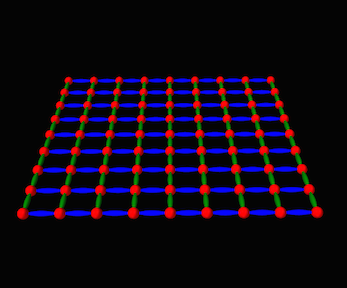
\includegraphics[]{images/NetDemo}
\else
 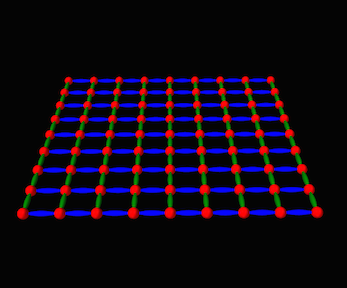
\includegraphics[width=3.75in]{images/NetDemo}
\fi
\end{center}
\caption{NetDemo model loaded into ArtiSynth.}
\label{NetDemo:fig}
\end{figure}

The {\tt build()} method and some of the supporting definitions for
this example are shown below.
%
\lstset{numbers=left}
\begin{lstlisting}[]
   protected double stiffness = 1000.0;   // spring stiffness
   protected double damping = 10.0;       // spring damping
   protected double maxForce = 5000.0;    // max force with excitation = 1
   protected double mass = 1.0;           // mass of each ball
   protected double widthx = 20.0;        // width of the net along x
   protected double widthy = 20.0;        // width of the net along y
   protected int numx = 8;                // num balls along x
   protected int numy = 8;                // num balls along y

   // custom component containers
   protected MechModel mech;
   protected PointList<Particle> balls;
   protected ComponentList<ModelComponent> springs;   
   protected RenderableComponentList<AxialSpring> greenSprings;
   protected RenderableComponentList<AxialSpring> blueSprings;

   private AxialSpring createSpring (
      PointList<Particle> parts, int idx0, int idx1) {
      // create a "muscle" spring connecting particles indexed by 'idx0' and
      // 'idx1' in the list 'parts'
      Muscle spr = new Muscle (parts.get(idx0), parts.get(idx1));
      spr.setMaterial (new SimpleAxialMuscle (stiffness, damping, maxForce));
      return spr;
   }

   public void build (String[] args) {

      // create MechModel and add to RootModel
      mech = new MechModel ("mech");
      mech.setGravity (0, 0, -980.0);
      mech.setPointDamping (1.0);
      addModel (mech);

      int nump = (numx+1)*(numy+1); // nump = total number of balls

      // create custom containers:
      balls = new PointList<Particle> (Particle.class, "balls");
      springs = new ComponentList<ModelComponent>(ModelComponent.class,"springs");
      greenSprings = new RenderableComponentList<AxialSpring> (
         AxialSpring.class, "greenSprings");
      blueSprings = new RenderableComponentList<AxialSpring> (
         AxialSpring.class, "blueSprings");

      // create balls in a grid pattern and add to the list 'balls'
      for (int i=0; i<=numx; i++) {
         for (int j=0; j<=numy; j++) {
            double x = widthx*(-0.5+i/(double)numx);
            double y = widthy*(-0.5+j/(double)numy);
            Particle p = new Particle (mass, x, y, /*z=*/0);
            balls.add (p);
            // fix balls along the edges parallel to y
            if (i == 0 || i == numx) {
               p.setDynamic (false);
            }
         }
      }

      // connect balls by green springs parallel to y
      for (int i=0; i<=numx; i++) {
         for (int j=0; j<numy; j++) {
            greenSprings.add (
               createSpring (balls, i*(numy+1)+j, i*(numy+1)+j+1));
         }
      }
      // connect balls by blue springs parallel to x
      for (int j=0; j<=numy; j++) {
         for (int i=0; i<numx; i++) {
            blueSprings.add (
               createSpring (balls, i*(numy+1)+j, (i+1)*(numy+1)+j));
         }
      }

      // add containers to the mechModel
      springs.add (greenSprings);
      springs.add (blueSprings);
      mech.add (balls);
      mech.add (springs);

      // set render properties for the components      
      RenderProps.setLineColor (greenSprings, new Color(0f, 0.5f, 0f));
      RenderProps.setLineColor (blueSprings, Color.BLUE);
      RenderProps.setSphericalPoints (mech, widthx/50.0, Color.RED);
      RenderProps.setCylindricalLines (mech, widthx/100.0, Color.BLUE);
   }
\end{lstlisting}
\lstset{numbers=none}
%
The {\tt build()} method begins by creating a {\tt MechModel} in the
usual way (lines 29-30). It then creates a net composed of a set of
balls arranged as a uniform grid in the x-y plane, connected by a set
of green colored springs running parallel to the y axis and a set of
blue colored springs running parallel to the x axis. These are
arranged into a component hierarchy of the form
%
\begin{lstlisting}[]
   balls
   springs
      greenSprings
      blueSprings
\end{lstlisting}
%
using containers created at lines 37-42. The balls are then created
and added to {\tt balls} (lines 45-56), the springs are created and
added to {\tt greenSprings} and {\tt blueSprings} (lines 59-71), and
the containers are added to the {\tt MechModel} at lines 74-77.
The balls along the edges parallel to the y axis are fixed.
Render properties are set at lines 80-83, with the colors for {\tt
greenSprings} and {\tt blueSprings} being explicitly set to dark green
and blue.

\begin{sideblock}
{\tt MechModel}, along with other classes derived from {\tt
ModelBase}, enforces {\it reference containment}. That means that all
components referenced by components within a {\tt MechModel} must
themselves be contained within the {\tt MechModel}.  This condition is
checked whenever a component is added directly to a {\tt MechModel} or
one of its ancestors. This means that the components must be added to
the {\tt MechModel} in an order that ensures any referenced components are
already present. For example, in the {\tt NetDemo} example above, adding the
particle list {\it after} the spring list would generate an error.
\end{sideblock}

To run this example in ArtiSynth, select {\sf All demos > tutorial >
NetDemo} from the {\sf Models} menu. The model should load and
initially appear as in Figure \ref{NetDemo:fig}.  Running the model
will cause the net to fall and sway under gravity. When the ArtiSynth
navigation panel is opened and expanded, the component hierarchy will
appear as in Figure \ref{NetDemoNav:fig}. While the standard
{\tt MechModel} containers are still present, they are not displayed
by default because they are empty.

\begin{figure}[ht]
\begin{center}
\iflatexml
 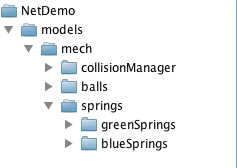
\includegraphics[]{images/NetDemoNav}
\else
 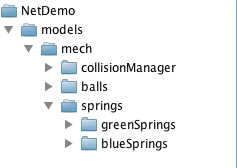
\includegraphics[width=2.25in]{images/NetDemoNav}
\fi
\end{center}
\caption{NetDemo components displayed in the ArtiSynth navigation panel.}
\label{NetDemoNav:fig}
\end{figure}

\subsection{Adding containers to other models}

In addition to {\tt MechModel}, application-defined containers can be
added to any model that inherits from
\javaclass[artisynth.core.modelbase]{ModelBase}. This includes {\tt
RootModel} and {\tt FemModel}. However, at the present time,
components added to such containers won't do anything, other than be
rendered in the viewer if they are
\javaclass[maspack.render]{Renderable}.

